%% ============================================================
% f2012_sichuan_sci_q18_wave.tex
%% 2012 四川卷（理科）第 18 题 f(x) 在一个周期内的图象，A 为最高点，B、C 为图象与 x 轴交点
%% 来源 PDF：普通高考/2012/2012四川理.pdf 第 2 页（印面 772）第 1 栏
%% 坐标取自原页矢量层（bp），原点为图区左上角 (230.0,160.0)，y 向下；AB、AC 为原页实线。
%% ============================================================
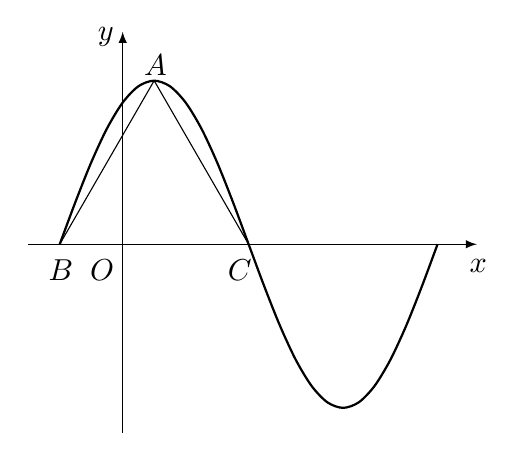
\begin{tikzpicture}[x=1bp,y=-1bp,
  every node/.style={inner sep=0,font=\fontsize{10.5pt}{12.6pt}\selectfont},
  line cap=butt, line join=miter]
  \draw[line width=0.3985bp] (6.215,85.234) -- (164.148,85.234);
  \fill[black] (167.734,85.234) .. controls (166.672,85.035) and (164.945,84.438) .. (163.75,83.738) -- (163.75,86.727) .. controls (164.945,86.031) and (166.672,85.434) .. (167.734,85.234);
  \draw[line width=0.3985bp] (40.219,153.242) -- (40.219,12.309);
  \fill[black] (40.219,8.727) .. controls (40.02,9.789) and (39.422,11.516) .. (38.727,12.707) -- (41.711,12.707) .. controls (41.016,11.516) and (40.418,9.789) .. (40.219,8.727);
  \draw[line width=0.797bp] (17.551,85.234) .. controls (17.551,85.234) and (21.645,74.074) .. (23.219,69.988) .. controls (24.789,65.902) and (27.313,59.449) .. (28.883,55.785) .. controls (30.457,52.121) and (32.98,46.578) .. (34.551,43.59) .. controls (36.125,40.598) and (38.645,36.344) .. (40.219,34.23) .. controls (41.793,32.113) and (44.313,29.441) .. (45.887,28.348) .. controls (47.457,27.25) and (49.98,26.34) .. (51.555,26.34) .. controls (53.125,26.34) and (55.648,27.25) .. (57.219,28.344) .. controls (58.793,29.438) and (61.316,32.113) .. (62.887,34.227) .. controls (64.461,36.34) and (66.98,40.594) .. (68.555,43.586) .. controls (70.129,46.578) and (72.648,52.121) .. (74.223,55.781) .. controls (75.793,59.445) and (78.316,65.902) .. (79.891,69.988) .. controls (81.461,74.07) and (83.984,81) .. (85.555,85.23) .. controls (87.129,89.457) and (89.652,96.387) .. (91.223,100.469) .. controls (92.797,104.555) and (95.316,111.012) .. (96.891,114.676) .. controls (98.465,118.34) and (100.984,123.883) .. (102.559,126.875) .. controls (104.129,129.863) and (106.652,134.117) .. (108.227,136.234) .. controls (109.797,138.352) and (112.32,141.023) .. (113.891,142.121) .. controls (115.465,143.215) and (117.988,144.129) .. (119.559,144.129) .. controls (121.133,144.129) and (123.652,143.219) .. (125.227,142.125) .. controls (126.801,141.031) and (129.32,138.355) .. (130.895,136.242) .. controls (132.465,134.129) and (134.988,129.875) .. (136.562,126.883) .. controls (138.133,123.895) and (140.656,118.352) .. (142.227,114.691) .. controls (143.801,111.027) and (146.324,104.57) .. (147.895,100.484) .. controls (149.469,96.398) and (153.562,85.242) .. (153.562,85.242);
  \draw[line width=0.3985bp] (17.551,85.234) -- (51.555,26.336) (51.555,26.336) -- (85.559,85.234);
  \node[anchor=base west] at (31.1,11.96) {$y$};
  \node[anchor=base west] at (47.72,24.64) {$A$};
  \node[anchor=base west] at (164.88,95.48) {$x$};
  \node[anchor=base west] at (13.4,98.13) {$B$};
  \node[anchor=base west] at (28.32,98.13) {$O$};
  \node[anchor=base west] at (77.86,98.13) {$C$};
\end{tikzpicture}
